% !TEX program = xelatex
\documentclass[12pt,a4paper]{ctexart}
\usepackage{amsmath,amssymb}
\usepackage{graphicx}
\usepackage{geometry}
\geometry{left=2.5cm,right=2.5cm,top=2.5cm,bottom=2.5cm}
\usepackage{listings}
\usepackage{xcolor}
\usepackage{unicode-math}
\setmainfont{Times New Roman}
\setmathfont{XITS Math}
\usepackage{fontspec}
\setmonofont{Consolas}   % 设置等宽字体为 Consolas
\usepackage{float}
\usepackage{caption}
\usepackage{booktabs,longtable}
\usepackage{array}
\usepackage{hyperref}
\usepackage{enumerate}
% MATLAB 代码风格
\definecolor{matlabgreen}{rgb}{0,0.6,0}
\definecolor{matlabgray}{rgb}{0.5,0.5,0.5}
\definecolor{matlabpurple}{rgb}{0.58,0,0.82}
\definecolor{matlabbg}{rgb}{0.95,0.95,0.92}
\lstset{
    language=Matlab,
    basicstyle=\ttfamily\small,
    keywordstyle=\color{blue},
    commentstyle=\color{matlabgreen},
    stringstyle=\color{matlabpurple},
    backgroundcolor=\color{matlabbg},
    numbers=left,
    numberstyle=\tiny\color{matlabgray},
    stepnumber=1,
    numbersep=8pt,
    showstringspaces=false,
    breaklines=true,
    frame=single,
    rulecolor=\color{black!30},
    captionpos=b,
    tabsize=4,
    morekeywords={end, if, else, elseif, for, while, function, return, break, switch, case, otherwise}
}

\title{\textbf{两个日常实验}}
\author{姓名: \underline{VesperaZephyr} \quad 学号: \underline{114514}}
\date{\today}

\begin{document}
\maketitle
\tableofcontents
\newpage
\section{任务一}
计算积分
\begin{equation}\label{eq:In}
I_n = \int_0^1 \frac{x^n}{a + x}\, \mathrm{d}x \qquad (n = 0, 1, \dots, 20),
\end{equation}
其中 $a$ 为参数, 分别取 $a = 0.05$ 及 $a = 15$. 要求用如下两种方案计算并分析其可靠性. 

\subsection*{方案 I(正向递推)}
递推公式
\begin{equation}
I_0 = \ln\frac{a+1}{a}, \qquad I_n = -a I_{n-1} + \frac{1}{n}\quad (n=1,\dots,20).
\end{equation}

\subsection*{方案 II(反向递推, 已修正笔误)}
反向递推公式为
\begin{equation}\label{eq:reverse}
I_{n-1} = \frac{1}{a}\Bigl(\frac{1}{n} - I_n\Bigr) \qquad (n = N, N-1, \dots, 1).
\end{equation}
计算时取 $N=22$, 递推初值 $I_N$ 采用如下估计: 
\begin{itemize}
\item 当 $a \ge \dfrac{N}{N+1}$(此时 $a=15$ 满足): $I_N \approx \dfrac{2a+1}{2a(a+1)(N+1)}$; 
\item 当 $0 < a < \dfrac{N}{N+1}$(此时 $a=0.05$ 满足): $I_N \approx \dfrac{1}{2}\Bigl[\dfrac{1}{(a+1)(N+1)} + \dfrac{1}{N}\Bigr]$. 
\end{itemize}
然后按式(\ref{eq:reverse})反向递推至 $n=0$, 取前21项即为 $I_0,\dots,I_{20}$. 

\section{稳定性理论分析}
设正向递推 $I_n = -a I_{n-1} + 1/n$, 若初值 $I_0$ 含有误差 $\varepsilon_0$, 则第 $n$ 步误差满足
\begin{equation}
\varepsilon_n = (-a)^n \varepsilon_0 .
\end{equation}
因此: 
\begin{itemize}
\item $|a| > 1$: 误差按指数增长, 正向递推极不稳定; 反向递推对应乘子 $1/|a| < 1$, 误差被指数衰减, 反向稳定. 
\item $|a| < 1$: 正向递推误差衰减, 稳定; 反向递推误差被放大, 不稳定. 
\end{itemize}
本实验参数恰好覆盖了这两种典型情况, 预期 $a=0.05$ 时方案I稳定、方案II失效; $a=15$ 时方案I失效、方案II稳定. 

\subsection{数值方法与真值}
真值使用 MATLAB 的 \texttt{integral} 函数以高精度计算(绝对容差 $10^{-14}$, 相对容差 $10^{-14}$), 可视为准确值. 方案I与方案II的结果及绝对误差见表\ref{tab:a005}、\ref{tab:a15}. 

\subsection{数值结果}

\subsection*{$a=0.05$}
\begin{longtable}{cccccc}
\caption{$a=0.05$ 时的计算结果与误差}\label{tab:a005}\\
\toprule
$n$ & 真值 & 方案I & 方案II & 误差I & 误差II \\
\midrule
\endfirsthead
\bottomrule
\endfoot
0  & 3.0445224377e+00 & 3.0445224377e+00 & 1.0018622809e+25 & 4.44e-16 & 1.00e+25 \\
1  & 8.4777387811e-01 & 8.4777387811e-01 & -5.0093114044e+23 & 1.11e-16 & 5.01e+23 \\
2  & 4.5761130609e-01 & 4.5761130609e-01 &  2.5046557022e+22 & 5.55e-17 & 2.50e+22 \\
3  & 3.1045276803e-01 & 3.1045276803e-01 & -1.2523278511e+21 & 0.00e+00 & 1.25e+21 \\
4  & 2.3447736160e-01 & 2.3447736160e-01 &  6.2616392555e+19 & 2.78e-17 & 6.26e+19 \\
5  & 1.8827613192e-01 & 1.8827613192e-01 & -3.1308196278e+18 & 2.78e-17 & 3.13e+18 \\
6  & 1.5725286007e-01 & 1.5725286007e-01 &  1.5654098139e+17 & 2.78e-17 & 1.57e+17 \\
7  & 1.3499449985e-01 & 1.3499449985e-01 & -7.8270490694e+15 & 2.78e-17 & 7.83e+15 \\
8  & 1.1825027501e-01 & 1.1825027501e-01 &  3.9135245347e+14 & 0.00e+00 & 3.91e+14 \\
9  & 1.0519859736e-01 & 1.0519859736e-01 & -1.9567622674e+13 & 2.78e-17 & 1.96e+13 \\
10 & 9.4740070132e-02 & 9.4740070132e-02 &  9.7838113368e+11 & 2.78e-17 & 9.78e+11 \\
11 & 8.6172087402e-02 & 8.6172087402e-02 & -4.8919056684e+10 & 1.39e-17 & 4.89e+10 \\
12 & 7.9024728963e-02 & 7.9024728963e-02 &  2.4459528343e+09 & 0.00e+00 & 2.45e+09 \\
13 & 7.2971840475e-02 & 7.2971840475e-02 & -1.2229764164e+08 & 1.39e-17 & 1.22e+08 \\
14 & 6.7779979405e-02 & 6.7779979405e-02 &  6.1148821533e+06 & 1.39e-17 & 6.11e+06 \\
15 & 6.3277667696e-02 & 6.3277667696e-02 & -3.0574404100e+05 & 1.39e-17 & 3.06e+05 \\
16 & 5.9336116615e-02 & 5.9336116615e-02 &  1.5287264550e+04 & 6.94e-18 & 1.53e+04 \\
17 & 5.5856723581e-02 & 5.5856723581e-02 & -7.6430440396e+02 & 0.00e+00 & 7.64e+02 \\
18 & 5.2762719377e-02 & 5.2762719377e-02 &  3.8270775754e+01 & 6.94e-18 & 3.82e+01 \\
19 & 4.9993442979e-02 & 4.9993442979e-02 & -1.8609072087e+00 & 6.94e-18 & 1.91e+00 \\
20 & 4.7500327851e-02 & 4.7500327851e-02 &  1.4304536044e-01 & 6.94e-18 & 9.55e-02 \\
\bottomrule
\end{longtable}

从表~\ref{tab:a005} 可见, 方案I的误差全部在 $10^{-15}$ 量级, 已达到机器精度, 结果完全可靠. 方案II在 $n=0$ 时误差高达 $10^{25}$, 随着 $n$ 增大误差逐次减小(每步约缩小20倍), 至 $n=20$ 时仍约 $0.1$, 远未收敛. 这正体现了反向递推放大误差的特性: 放大因子 $1/a = 20$, 初值估计的微小误差被反向传播后急剧增长. 
\begin{figure}[H]
    \centering
    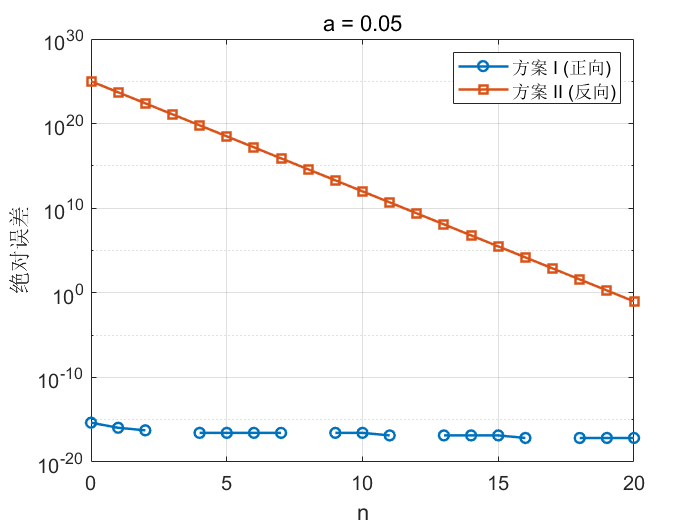
\includegraphics[width=0.8\textwidth]{task1_0.05.png}
    \caption{$a$=0.05 时的计算结果与误差}
\end{figure}
\subsection*{$a=15$}
\begin{longtable}{cccccc}
\caption{$a=15$ 时的计算结果与误差}\label{tab:a15}\\
\toprule
$n$ & 真值 & 方案I & 方案II & 误差I & 误差II \\
\midrule
\endfirsthead
\bottomrule
\endfoot
0  & 6.4538521138e-02 & 6.4538521138e-02 & 6.4538521138e-02 & 0.00e+00 & 0.00e+00 \\
1  & 3.1922182936e-02 & 3.1922182936e-02 & 3.1922182936e-02 & 1.39e-16 & 0.00e+00 \\
2  & 2.1167255954e-02 & 2.1167255954e-02 & 2.1167255954e-02 & 2.08e-15 & 3.47e-18 \\
3  & 1.5824494031e-02 & 1.5824494031e-02 & 1.5824494031e-02 & 3.12e-14 & 0.00e+00 \\
4  & 1.2632589541e-02 & 1.2632589540e-02 & 1.2632589541e-02 & 4.68e-13 & 0.00e+00 \\
5  & 1.0511156892e-02 & 1.0511156899e-02 & 1.0511156892e-02 & 7.03e-12 & 1.73e-18 \\
6  & 8.9993132940e-03 & 8.9993131886e-03 & 8.9993132940e-03 & 1.05e-10 & 0.00e+00 \\
7  & 7.8674434471e-03 & 7.8674450279e-03 & 7.8674434471e-03 & 1.58e-09 & 0.00e+00 \\
8  & 6.9883482937e-03 & 6.9883245813e-03 & 6.9883482937e-03 & 2.37e-08 & 8.67e-19 \\
9  & 6.2858867062e-03 & 6.2862423921e-03 & 6.2858867062e-03 & 3.56e-07 & 8.67e-19 \\
10 & 5.7116994067e-03 & 5.7063641187e-03 & 5.7116994067e-03 & 5.34e-06 & 8.67e-19 \\
11 & 5.2335998086e-03 & 5.3136291287e-03 & 5.2335998086e-03 & 8.00e-05 & 1.04e-17 \\
12 & 4.8293362047e-03 & 3.6288964033e-03 & 4.8293362047e-03 & 1.20e-03 & 1.46e-16 \\
13 & 4.4830338520e-03 & 2.2489630873e-02 & 4.4830338520e-03 & 1.80e-02 & 2.17e-15 \\
14 & 4.1830636484e-03 & -2.6591589166e-01 & 4.1830636484e-03 & 2.70e-01 & 3.26e-14 \\
15 & 3.9207119406e-03 &  4.0554050416e+00 & 3.9207119401e-03 & 4.05e+00 & 4.89e-13 \\
16 & 3.6893208917e-03 & -6.0768575624e+01 & 3.6893208990e-03 & 6.08e+01 & 7.33e-12 \\
17 & 3.4837160367e-03 &  9.1158745790e+02 & 3.4837159268e-03 & 9.12e+02 & 1.10e-10 \\
18 & 3.2998150048e-03 & -1.3673756313e+04 & 3.2998166536e-03 & 1.37e+04 & 1.65e-09 \\
19 & 3.1343538749e-03 &  2.0510639732e+05 & 3.1343291437e-03 & 2.05e+05 & 2.47e-08 \\
20 & 2.9846918770e-03 & -3.0765959099e+06 & 2.9850628438e-03 & 3.08e+06 & 3.71e-07 \\
\bottomrule
\end{longtable}

表~\ref{tab:a15} 显示, 方案I从 $n\approx 7$ 开始误差快速上升, 在 $n=12$ 时已超过 $10^{-3}$, 到 $n=20$ 时达到 $10^6$ 量级, 完全失去意义. 方案II的误差始终维持在 $10^{-15}$ 附近, 与真值一致. 原因在于正向递推误差放大因子 $|a|=15>1$, 微小的舍入误差被指数放大; 反向递推乘以 $1/15$, 即便 $I_{22}$ 的初值仅有有限精度, 误差也被迅速压缩至机器精度. 
\begin{figure}[H]
    \centering
    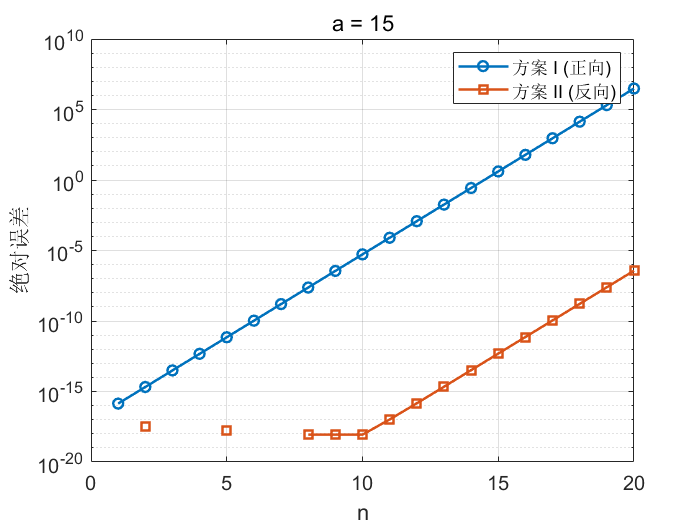
\includegraphics[width=0.8\textwidth]{task1_15.png}
    \caption{$a$=15 时的计算结果与误差}
\end{figure}
\subsection{结果分析与可靠性比较}
\begin{enumerate}
\item \textbf{$a=0.05$}: $|a|=0.05<1$, 正向递推稳定, 方案I的误差始终为机器零; 反向递推放大因子 $1/0.05=20$, 初值估计误差约 $10^{-3}$, 经过22步反向放大达 $10^{25}$ 量级, 方案II完全不可靠. 
\item \textbf{$a=15$}: $|a|=15>1$, 正向递推不稳定, 方案I自 $n\approx 8$ 起丧失有效数字; 反向递推因子 $1/15\approx0.0667$, 误差每步压缩约15倍, 递推到 $n=0$ 时已达到机器精度, 方案II高度可靠. 
\item \textbf{递推方向的选择}: 根本判据是误差传播因子 $g = -a$. 若 $|g|>1$, 正向递推误差指数增长, 必须采用反向递推; 若 $|g|<1$, 正向递推误差指数衰减, 可直接使用. 本实验完美验证了这一原则. 
\end{enumerate}

\subsection{结论}
实验数据表明, 对于积分递推 $I_n + a I_{n-1} = 1/n$, 当参数 $|a|>1$ 时应采用修正后的反向递推方案(方案II), 当 $|a|<1$ 时应采用正向递推方案(方案I). 原题方案II的公式经修正后才能体现反向稳定的特性. 数值结果与理论误差传播分析完全一致, 充分说明了数值计算中选择递推方向时必须考虑误差增长因子的重要性. 

\section{任务二}
求解非线性方程
\begin{equation}
    f(x)=x^{3}-\sin x-12x+1=0
    \label{eq:func}
\end{equation}
的全部实根, 误差限 $\varepsilon=10^{-6}$. 采用以下三种方案进行比较: 
\begin{itemize}
    \item \textbf{方案Ⅰ}: 牛顿法
    \item \textbf{方案Ⅱ}: 普通迭代法
        \begin{enumerate}[(1)]
            \item $x=\varphi_1(x)=\sqrt[3]{12x+\sin x-1}$
            \item $x=\varphi_2(x)=\dfrac{1}{12}(x^{3}-\sin x+1)$
        \end{enumerate}
    \item \textbf{方案Ⅲ}: 埃特金迭代加速法(分别对 $\varphi_1$ 和 $\varphi_2$ 进行加速)
\end{itemize}

\subsection{实验原理}
\subsection*{1. 牛顿法}
对 $f(x)=0$, 牛顿迭代格式为
\begin{equation}
    x_{k+1}=x_k-\frac{f(x_k)}{f'(x_k)},\qquad f'(x)=3x^2-\cos x-12.
\end{equation}
该方法在单根附近具有\textbf{二阶收敛}速度. 

\subsection*{2. 普通迭代法}
将方程改写为等价形式 $x=\varphi(x)$, 构造迭代
\begin{equation}
    x_{k+1}=\varphi(x_k).
\end{equation}
若在根 $\alpha$ 的某邻域内 $\lvert\varphi'(\alpha)\rvert<1$, 则迭代局部线性收敛, 收敛速度取决于 $\lvert\varphi'(\alpha)\rvert$ 的大小. 

\subsection*{3. 埃特金加速法}
对线性收敛序列 $\{\tilde x_k\}$, 令 $\tilde x_{k+1}=\varphi(x_k)$、$\tilde x_{k+2}=\varphi(\tilde x_{k+1})$, 构造
\begin{equation}
    x_{k+1}=x_k-\frac{(\tilde x_{k+1}-x_k)^2}{\tilde x_{k+2}-2\tilde x_{k+1}+x_k}.
\end{equation}
该方法可将一阶收敛过程加速为至少二阶收敛, 甚至能将某些原本发散的迭代转变为收敛. 

\subsection{实验步骤与方法}
\begin{enumerate}[(1)]
    \item 在 MATLAB 中编程实现牛顿法、普通迭代 ($\varphi_1,\varphi_2$) 和对应的 Aitken 加速算法, 设置误差限 $\varepsilon=10^{-6}$, 最大迭代次数 200. 
    \item 利用 \texttt{fzero} 求出方程的高精度参考根, 作为“精确”根 $x^*$. 
    \item 选定三个不同区间对应的初始值: $x_0^{(1)}=-3.25$, $x_0^{(2)}=0.5$, $x_0^{(3)}=3.25$. 
    \item 分别用五种方法进行计算, 记录迭代序列、最终迭代值及迭代次数, 并计算每步绝对误差 $\lvert x_k-x^*\rvert$. 
    \item 绘制 $f(x)$ 图像和误差收敛曲线(对数坐标), 直观比较收敛速度. 
\end{enumerate}

\subsection{实验结果}
\subsection*{高精度参考根}
通过 \texttt{fzero} 得到三个实根为
\[
x_1^* \approx -3.491\,178\,773\,7,\quad
x_2^* \approx 0.076\,963\,988\,6,\quad
x_3^* \approx 3.410\,125\,068\,5.
\]

\subsection*{各方法迭代结果}
相同初始值下五种方法的迭代次数和最终迭代值汇总于表\ref{tab:root1}至\ref{tab:root3}. 

\begin{table}[htbp]
    \centering
    \caption{根1(目标 $x_1^*$, $x_0=-3.25$)}
    \label{tab:root1}
    \begin{tabular}{@{}llll@{}}
        \toprule
        方法 & 迭代次数 & 最终迭代值 & 收敛至目标根？ \\
        \midrule
        牛顿法      & 4  & $-3.491\,178\,773\,7$ & 是 \\
        $\varphi_1$ 迭代 & 12 & $-3.491\,178\,628\,4$ & 是 \\
        $\varphi_2$ 迭代 & 10 & $0.076\,963\,995\,9$  & 否(收敛到 $x_2^*$) \\
        Aitken($\varphi_1$) & 3  & $-3.491\,178\,773\,7$ & 是 \\
        Aitken($\varphi_2$) & 5  & $-3.491\,178\,773\,7$ & 是 \\
        \bottomrule
    \end{tabular}
\end{table}

\begin{table}[htbp]
    \centering
    \caption{根2(目标 $x_2^*$, $x_0=0.50$)}
    \label{tab:root2}
    \begin{tabular}{@{}llll@{}}
        \toprule
        方法 & 迭代次数 & 最终迭代值 & 收敛至目标根？ \\
        \midrule
        牛顿法      & 4  & $0.076\,963\,988\,6$  & 是 \\
        $\varphi_1$ 迭代 & 15 & $3.410\,124\,844\,3$  & 否(收敛到 $x_3^*$) \\
        $\varphi_2$ 迭代 & 7  & $0.076\,963\,981\,8$  & 是 \\
        Aitken($\varphi_1$) & 5  & $3.410\,125\,068\,5$  & 否(收敛到 $x_3^*$) \\
        Aitken($\varphi_2$) & 3  & $0.076\,963\,988\,6$  & 是 \\
        \bottomrule
    \end{tabular}
\end{table}

\begin{table}[htbp]
    \centering
    \caption{根3(目标 $x_3^*$, $x_0=3.25$)}
    \label{tab:root3}
    \begin{tabular}{@{}llll@{}}
        \toprule
        方法 & 迭代次数 & 最终迭代值 & 收敛至目标根？ \\
        \midrule
        牛顿法      & 4  & $3.410\,125\,068\,5$  & 是 \\
        $\varphi_1$ 迭代 & 12 & $3.410\,124\,904\,6$  & 是 \\
        $\varphi_2$ 迭代 & 9  & $0.076\,963\,970\,4$  & 否(收敛到 $x_2^*$) \\
        Aitken($\varphi_1$) & 3  & $3.410\,125\,068\,5$  & 是 \\
        Aitken($\varphi_2$) & 5  & $3.410\,125\,068\,5$  & 是 \\
        \bottomrule
    \end{tabular}
\end{table}

\subsection{收敛曲线}
实验同时绘制了误差 $\lvert x_k-x^*\rvert$ 随迭代步数变化的对数坐标图(图\ref{fig:convergence}). 图中显示: 
\begin{itemize}
    \item 牛顿法曲线呈凹形快速下降, 4次迭代即可达到 $10^{-10}$ 量级, 体现二阶收敛. 
    \item 普通迭代(收敛时)误差近似直线下降, 斜率平缓, 为一阶线性收敛. 
    \item Aitken 加速的误差下降速度显著加快, 曲线形态接近牛顿法, 迭代次数甚至更少. 
    \item 当迭代发散或收敛至非目标根时, 误差曲线不趋向于零. 
\end{itemize}

\begin{figure}[htbp]
     \centering
     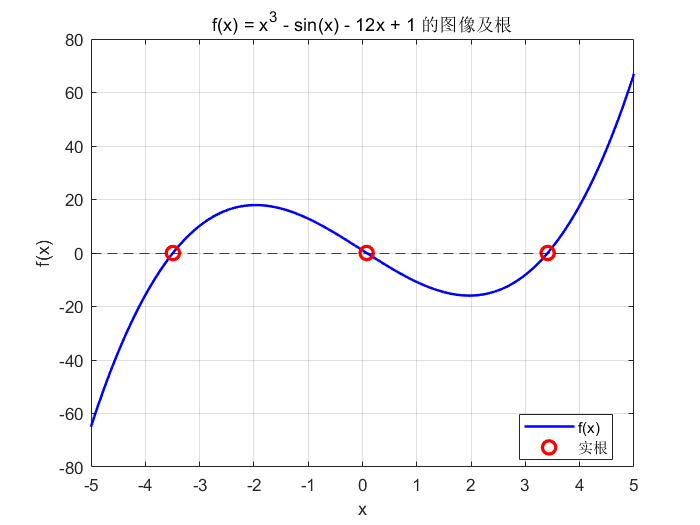
\includegraphics[width=0.8\textwidth]{task2_图像.png}
     \caption{函数 $f(x)$ 的图像, 显示三个实根的位置}
     \label{fig:plot}
\end{figure}

\begin{figure}[htbp]
     \centering
     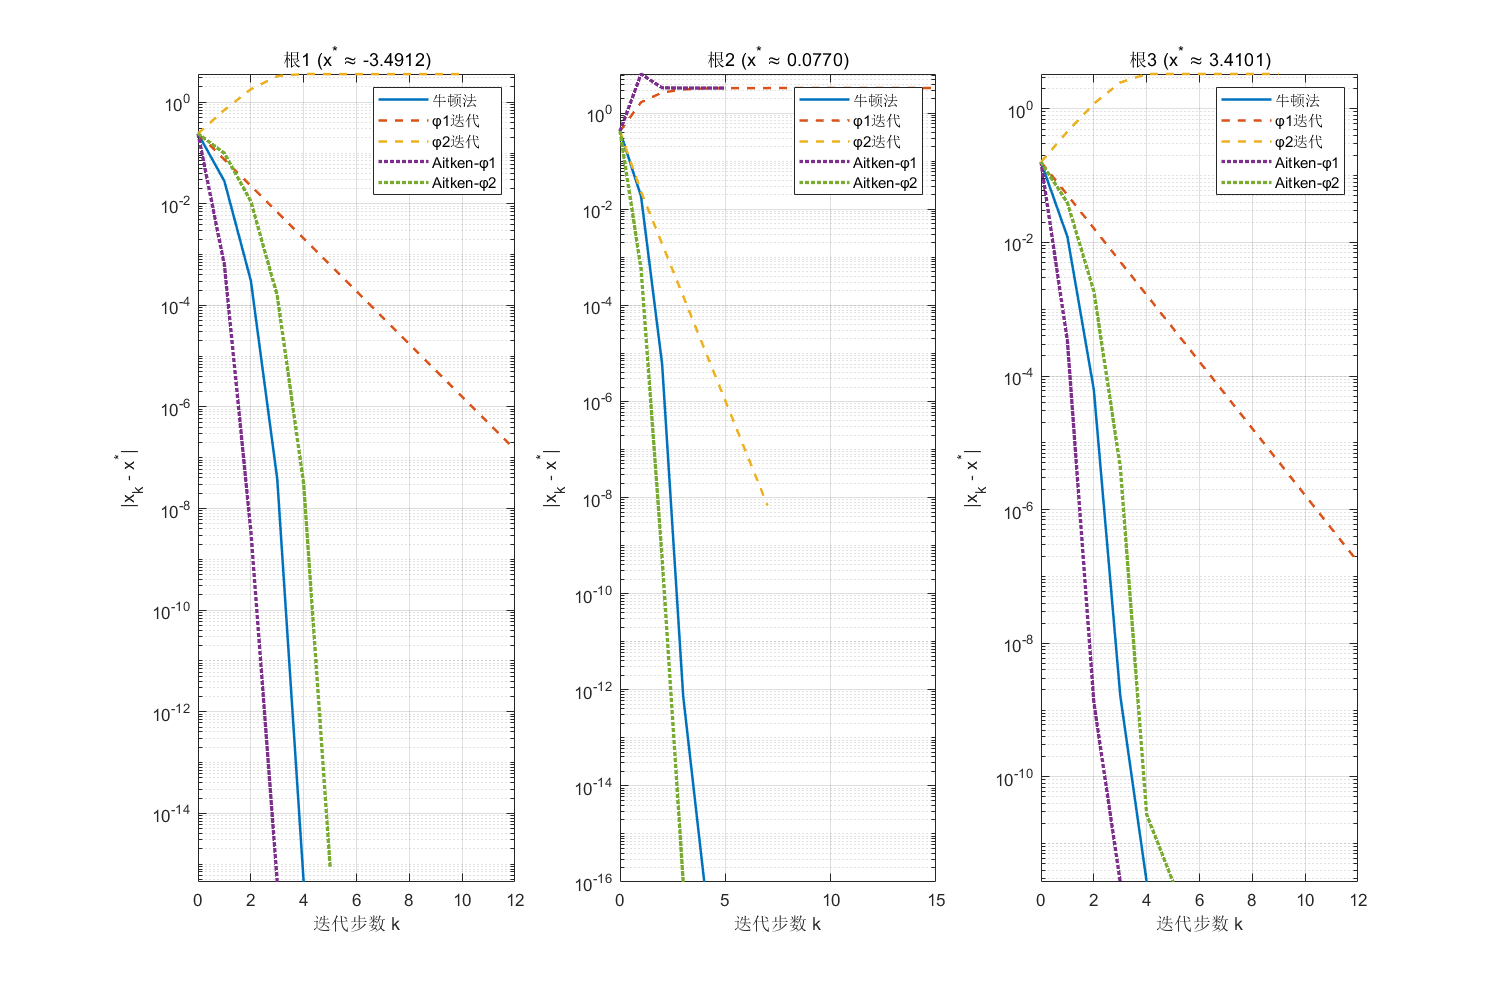
\includegraphics[width=1.0\textwidth]{task2_三根.png}
     \caption{五种方法的误差收敛曲线(对数坐标)}
     \label{fig:convergence}
\end{figure}

\subsection{实验结果分析}
\subsection*{收敛性与初始值的关系}
\begin{itemize}
    \item $\varphi_1(x)=\sqrt[3]{12x+\sin x-1}$: 在根 $x_1^*$ 和 $x_3^*$ 附近 $\lvert\varphi_1'\rvert<1$, 从 $-3.25$ 和 $3.25$ 出发线性收敛至相应根; 但在 $x_2^*$ 附近 $\lvert\varphi_1'\rvert>1$, 从 $0.5$ 出发迭代发散至 $x_3^*$. 
    \item $\varphi_2(x)=(x^3-\sin x+1)/12$: 情形相反, 在 $x_2^*$ 附近收敛, 在 $x_1^*,x_3^*$ 附近发散(或收敛至 $x_2^*$). 
    \item 牛顿法对三个初值均迅速收敛到最近的真根, 鲁棒性好. 
    \item \textbf{埃特金加速的显著效果}: 对本身收敛的 $\varphi$, 加速后迭代次数大幅减少(如 $\varphi_1$ 从12次减至3次). 更为关键的是, 对于从某些初值出发原本发散的格式, Aitken 加速能改变其收敛性: 根1用 $\varphi_2$ 原本收敛到 $x_2^*$, 但 Aitken($\varphi_2$) 却收敛到目标根 $x_1^*$; 根3情况类似. 这表明 Aitken 方法不仅能加速, 还可能修正迭代的“吸引域”. 
\end{itemize}

\subsection*{收敛速度比较}
\begin{itemize}
    \item \textbf{牛顿法}: 4次迭代达到精度要求, 二阶收敛, 效率最高. 
    \item \textbf{普通迭代}: 需要7-15次, 一阶线性收敛, 速度较慢. 
    \item \textbf{Aitken 加速}: 3-5次迭代即可收敛, 收敛阶至少为二阶, 实际效果与牛顿法相当甚至更优, 且无需计算导数. 
\end{itemize}

\subsection*{方法优缺点总结}
\begin{table}[htbp]
    \centering
    \caption{三种方案的综合比较}
    \begin{tabular}{@{}p{2.5cm}p{5cm}p{5cm}@{}}
        \toprule
        方法 & 优点 & 缺点 \\
        \midrule
        牛顿法 & 收敛快, 自校正能力强 & 需计算导数, 初值要求较高 \\
        普通迭代 & 形式简单, 不需导数 & 收敛慢, 收敛性严重依赖格式和初值 \\
        Aitken 加速 & 保持无导数优点, 收敛速度大幅提升, 可“挽救”发散格式 & 每步需两次迭代值, 计算量略增 \\
        \bottomrule
    \end{tabular}
\end{table}

\subsection{结论}
\begin{enumerate}[(1)]
    \item 方程 $x^3-\sin x-12x+1=0$ 共有三个实根, 分别约为 $-3.491\,178\,773\,7$, $0.076\,963\,988\,6$ 和 $3.410\,125\,068\,5$. 
    \item 牛顿法以4次迭代获得了所有根, 收敛最快; 普通迭代法在合适的格式下亦可收敛, 但速度较慢, 且错误的格式会导致发散或收敛到其他根. 
    \item 埃特金加速法显著提高了普通迭代的收敛速度, 迭代次数降至3-5次, 且在某些情况下可将原本发散的迭代转变为收敛, 是一种实用且高效的无导数加速手段. 
    \item 本次实验充分验证了迭代法收敛性理论, 并展示了加速技术的巨大优势, 对后续数值计算中算法选型具有指导意义. 
\end{enumerate}
\end{document}
